\section{Урвуу инженерчлэл: "Auftragsverwaltung" систем дэх зохиомжийн үлгэр загварууд}
Энэ хэсэгт Жава технологийг ашиглан хэрэгжүүлсэн бараа захиалгийг зохицуулах Герман нэршлийн конвенцтэй "Auftragsverwaltung" систем дээр урвуу инженерчлэлийн аргачлалаар програм хангамжийн зохиомжийн үлгэр загваруудыг уг системд хэрхэн ашигласан байгааг олж тогтооно.

\subsection{Системийн статик загвар}
Системийн классын диаграмыг гаргахын тулд Eclipse IDE дээрх PlantUML програм хангам -жийн багажыг ашигласан. Гэвч энэ багаж нь классууд хоорондын холбоосуудыг, тухайлбал бүрдмэл, нийлмэл зэрэг холбоог оновчтой гаргаж чадаагүй. Юуны түрүүнд энэ системийн гарчиглалт нь Герман хэл дээр хийгдсэн учир тодорхой үгсийн Герман–Англи нэр томьёоны тайлбарыг гаргах шаардлага үүссэн. Жишээ нь, Auftragsverwaltung нь "Order management" буюу "Захиалгын удирдлага", Auftrag нь "Order" буюу "Захиалга", Kunde нь "Customer" буюу "Харилцагч" гэх мэт. Үүний дараа системийн бүх классын нэрсийг жагсааж, тэдгээрийн хоорондын холбоосуудыг гаргаж авсан. Эцэст нь, холбоосуудын төрлийг тодорхойлж, UML классын диаграмыг гаргасан.

% \begin{figure}
% 	\centering
% 	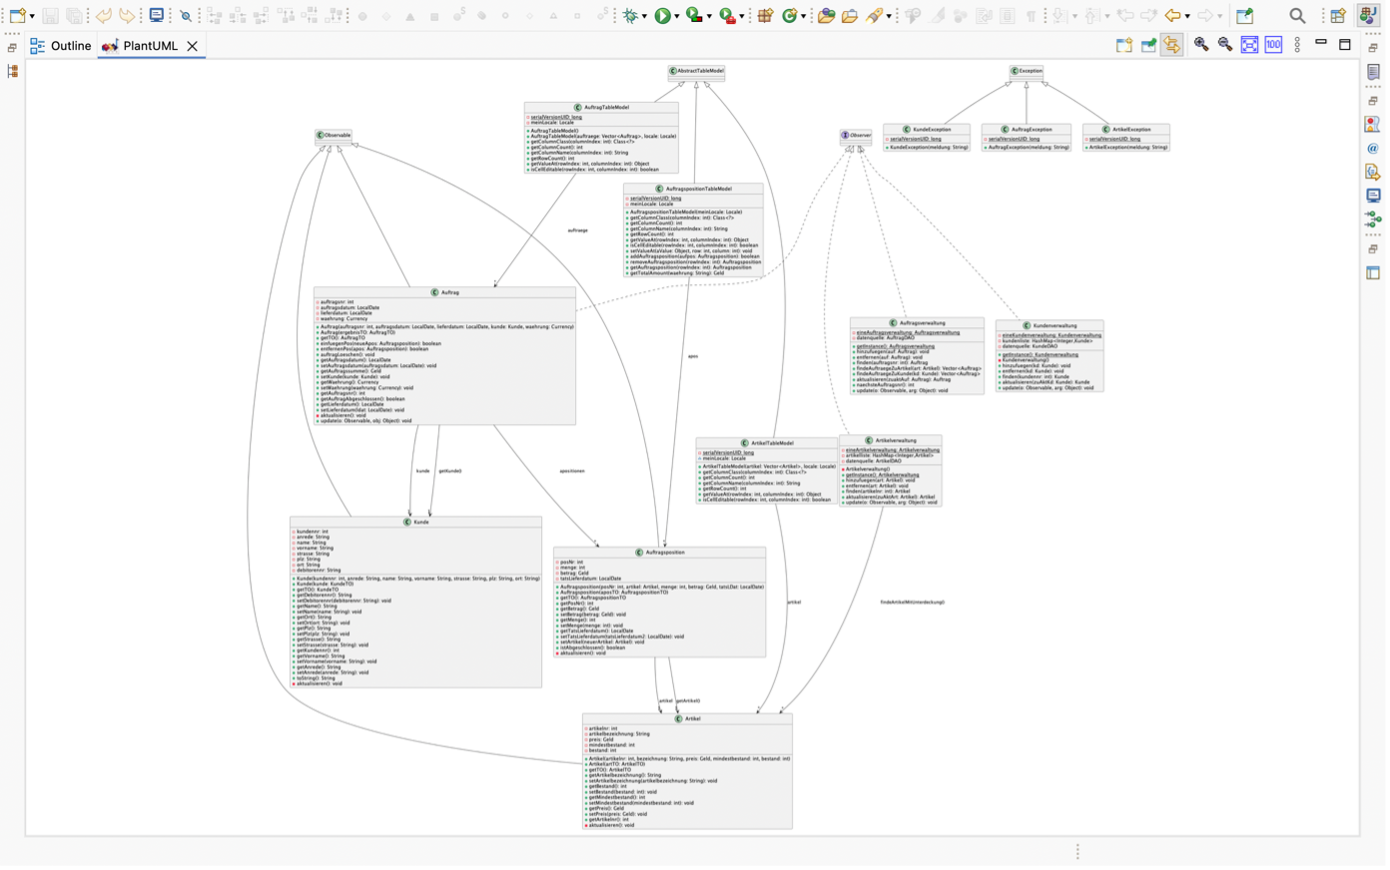
\includegraphics[width=15cm]{images/plantuml.png}
% 	\caption{UML багажаар үүсгэсэн "Applicationlogic" багцын классын диаграм}
% 	\label{fig:hhe}
% \end{figure}

Холбоосуудын төрлийг тодорхойлохын тулд класс тус бүрийн устгагчийн хэрэгжүүлэлтийг ажигласан. Жишээ нь, Order (Aufrag), OrderItem (Aufragsposition) классуудын хувьд Order классын объектийг устгах үед OrderItem классын объектуудаас бүрдсэн векторыг устгаж байна. Иймд Order, OrderItem классууд хоорондоо нийлмэл холбоотой гэж дүгнэлээ.
\begin{lstlisting}
public boolean entfernenPos(Auftragsposition apos)
{
    boolean rc = apositionen.remove(apos);
    if (rc)
        this.aktualisieren();
    return rc;
}

/**
 * L�scht einen vorhandenen Auftrag.
 */
public void auftragLoeschen()
{
    Iterator<Auftragsposition> positionen =
            apositionen.iterator();
    while (positionen.hasNext())
    {
        entfernenPos(positionen.next());
    }
}
\end{lstlisting}


\begin{lstlisting}
\end{lstlisting}